\documentclass[twoside]{book}

% Packages required by doxygen
\usepackage{fixltx2e}
\usepackage{calc}
\usepackage{doxygen}
\usepackage[export]{adjustbox} % also loads graphicx
\usepackage{graphicx}
\usepackage[utf8]{inputenc}
\usepackage{makeidx}
\usepackage{multicol}
\usepackage{multirow}
\PassOptionsToPackage{warn}{textcomp}
\usepackage{textcomp}
\usepackage[nointegrals]{wasysym}
\usepackage[table]{xcolor}

% Font selection
\usepackage[T1]{fontenc}
\usepackage[scaled=.90]{helvet}
\usepackage{courier}
\usepackage{amssymb}
\usepackage{sectsty}
\renewcommand{\familydefault}{\sfdefault}
\allsectionsfont{%
  \fontseries{bc}\selectfont%
  \color{darkgray}%
}
\renewcommand{\DoxyLabelFont}{%
  \fontseries{bc}\selectfont%
  \color{darkgray}%
}
\newcommand{\+}{\discretionary{\mbox{\scriptsize$\hookleftarrow$}}{}{}}

% Page & text layout
\usepackage{geometry}
\geometry{%
  a4paper,%
  top=2.5cm,%
  bottom=2.5cm,%
  left=2.5cm,%
  right=2.5cm%
}
\tolerance=750
\hfuzz=15pt
\hbadness=750
\setlength{\emergencystretch}{15pt}
\setlength{\parindent}{0cm}
\setlength{\parskip}{3ex plus 2ex minus 2ex}
\makeatletter
\renewcommand{\paragraph}{%
  \@startsection{paragraph}{4}{0ex}{-1.0ex}{1.0ex}{%
    \normalfont\normalsize\bfseries\SS@parafont%
  }%
}
\renewcommand{\subparagraph}{%
  \@startsection{subparagraph}{5}{0ex}{-1.0ex}{1.0ex}{%
    \normalfont\normalsize\bfseries\SS@subparafont%
  }%
}
\makeatother

% Headers & footers
\usepackage{fancyhdr}
\pagestyle{fancyplain}
\fancyhead[LE]{\fancyplain{}{\bfseries\thepage}}
\fancyhead[CE]{\fancyplain{}{}}
\fancyhead[RE]{\fancyplain{}{\bfseries\leftmark}}
\fancyhead[LO]{\fancyplain{}{\bfseries\rightmark}}
\fancyhead[CO]{\fancyplain{}{}}
\fancyhead[RO]{\fancyplain{}{\bfseries\thepage}}
\fancyfoot[LE]{\fancyplain{}{}}
\fancyfoot[CE]{\fancyplain{}{}}
\fancyfoot[RE]{\fancyplain{}{\bfseries\scriptsize Generated by Doxygen }}
\fancyfoot[LO]{\fancyplain{}{\bfseries\scriptsize Generated by Doxygen }}
\fancyfoot[CO]{\fancyplain{}{}}
\fancyfoot[RO]{\fancyplain{}{}}
\renewcommand{\footrulewidth}{0.4pt}
\renewcommand{\chaptermark}[1]{%
  \markboth{#1}{}%
}
\renewcommand{\sectionmark}[1]{%
  \markright{\thesection\ #1}%
}

% Indices & bibliography
\usepackage{natbib}
\usepackage[titles]{tocloft}
\setcounter{tocdepth}{3}
\setcounter{secnumdepth}{5}
\makeindex

% Hyperlinks (required, but should be loaded last)
\usepackage{ifpdf}
\ifpdf
  \usepackage[pdftex,pagebackref=true]{hyperref}
\else
  \usepackage[ps2pdf,pagebackref=true]{hyperref}
\fi
\hypersetup{%
  colorlinks=true,%
  linkcolor=blue,%
  citecolor=blue,%
  unicode%
}

% Custom commands
\newcommand{\clearemptydoublepage}{%
  \newpage{\pagestyle{empty}\cleardoublepage}%
}

\usepackage{caption}
\captionsetup{labelsep=space,justification=centering,font={bf},singlelinecheck=off,skip=4pt,position=top}

%===== C O N T E N T S =====

\begin{document}

% Titlepage & ToC
\hypersetup{pageanchor=false,
             bookmarksnumbered=true,
             pdfencoding=unicode
            }
\pagenumbering{alph}
\begin{titlepage}
\vspace*{7cm}
\begin{center}%
{\Large Uno }\\
\vspace*{1cm}
{\large Generated by Doxygen 1.8.13}\\
\end{center}
\end{titlepage}
\clearemptydoublepage
\pagenumbering{roman}
\tableofcontents
\clearemptydoublepage
\pagenumbering{arabic}
\hypersetup{pageanchor=true}

%--- Begin generated contents ---
\chapter{Class Index}
\section{Class List}
Here are the classes, structs, unions and interfaces with brief descriptions\+:\begin{DoxyCompactList}
\item\contentsline{section}{\hyperlink{classScanner}{Scanner} }{\pageref{classScanner}}{}
\item\contentsline{section}{\hyperlink{classToken}{Token} }{\pageref{classToken}}{}
\item\contentsline{section}{\hyperlink{classUno}{Uno} }{\pageref{classUno}}{}
\end{DoxyCompactList}

\chapter{File Index}
\section{File List}
Here is a list of all files with brief descriptions\+:\begin{DoxyCompactList}
\item\contentsline{section}{src/\hyperlink{main_8cpp}{main.\+cpp} \\*\hyperlink{classUno}{Uno} language interpreter.  uno \mbox{[}path\+\_\+to\+\_\+scritp\mbox{]} if a path is given, it\textquotesingle{}s code is run. if uno is called without arguments, an interactive R\+PL is launched }{\pageref{main_8cpp}}{}
\item\contentsline{section}{src/\hyperlink{Scanner_8cpp}{Scanner.\+cpp} }{\pageref{Scanner_8cpp}}{}
\item\contentsline{section}{src/\hyperlink{Scanner_8h}{Scanner.\+h} }{\pageref{Scanner_8h}}{}
\item\contentsline{section}{src/\hyperlink{Token_8cpp}{Token.\+cpp} }{\pageref{Token_8cpp}}{}
\item\contentsline{section}{src/\hyperlink{Token_8h}{Token.\+h} }{\pageref{Token_8h}}{}
\item\contentsline{section}{src/\hyperlink{Uno_8cpp}{Uno.\+cpp} }{\pageref{Uno_8cpp}}{}
\item\contentsline{section}{src/\hyperlink{Uno_8h}{Uno.\+h} }{\pageref{Uno_8h}}{}
\end{DoxyCompactList}

\chapter{Class Documentation}
\hypertarget{classScanner}{}\section{Scanner Class Reference}
\label{classScanner}\index{Scanner@{Scanner}}


{\ttfamily \#include $<$Scanner.\+h$>$}

\subsection*{Public Member Functions}
\begin{DoxyCompactItemize}
\item 
\hyperlink{classScanner_a149fab95f2549cf7d8405c79190c9903}{Scanner} (std\+::string src)
\item 
std\+::list$<$ \hyperlink{classToken}{Token} $>$ \hyperlink{classScanner_aefda786435557ddefd93791e890adfe6}{get\+Tokens} (void)
\item 
void \hyperlink{classScanner_a38e0f484bb3539944d6809c552f1da0b}{scan\+Tokens} (void)
\end{DoxyCompactItemize}


\subsection{Detailed Description}


Definition at line 7 of file Scanner.\+h.



\subsection{Constructor \& Destructor Documentation}
\mbox{\Hypertarget{classScanner_a149fab95f2549cf7d8405c79190c9903}\label{classScanner_a149fab95f2549cf7d8405c79190c9903}} 
\index{Scanner@{Scanner}!Scanner@{Scanner}}
\index{Scanner@{Scanner}!Scanner@{Scanner}}
\subsubsection{\texorpdfstring{Scanner()}{Scanner()}}
{\footnotesize\ttfamily Scanner\+::\+Scanner (\begin{DoxyParamCaption}\item[{std\+::string}]{src }\end{DoxyParamCaption})\hspace{0.3cm}{\ttfamily [explicit]}}



Definition at line 10 of file Scanner.\+cpp.



\subsection{Member Function Documentation}
\mbox{\Hypertarget{classScanner_aefda786435557ddefd93791e890adfe6}\label{classScanner_aefda786435557ddefd93791e890adfe6}} 
\index{Scanner@{Scanner}!get\+Tokens@{get\+Tokens}}
\index{get\+Tokens@{get\+Tokens}!Scanner@{Scanner}}
\subsubsection{\texorpdfstring{get\+Tokens()}{getTokens()}}
{\footnotesize\ttfamily std\+::list$<$ \hyperlink{classToken}{Token} $>$ Scanner\+::get\+Tokens (\begin{DoxyParamCaption}\item[{void}]{ }\end{DoxyParamCaption})}



Definition at line 34 of file Scanner.\+cpp.

Here is the caller graph for this function\+:
\nopagebreak
\begin{figure}[H]
\begin{center}
\leavevmode
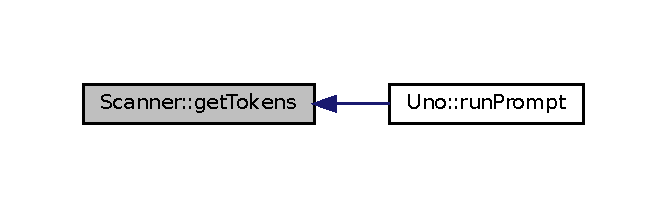
\includegraphics[width=320pt]{classScanner_aefda786435557ddefd93791e890adfe6_icgraph}
\end{center}
\end{figure}
\mbox{\Hypertarget{classScanner_a38e0f484bb3539944d6809c552f1da0b}\label{classScanner_a38e0f484bb3539944d6809c552f1da0b}} 
\index{Scanner@{Scanner}!scan\+Tokens@{scan\+Tokens}}
\index{scan\+Tokens@{scan\+Tokens}!Scanner@{Scanner}}
\subsubsection{\texorpdfstring{scan\+Tokens()}{scanTokens()}}
{\footnotesize\ttfamily void Scanner\+::scan\+Tokens (\begin{DoxyParamCaption}\item[{void}]{ }\end{DoxyParamCaption})}



Definition at line 38 of file Scanner.\+cpp.

Here is the call graph for this function\+:
\nopagebreak
\begin{figure}[H]
\begin{center}
\leavevmode
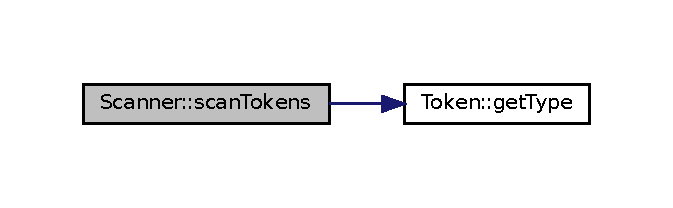
\includegraphics[width=323pt]{classScanner_a38e0f484bb3539944d6809c552f1da0b_cgraph}
\end{center}
\end{figure}
Here is the caller graph for this function\+:
\nopagebreak
\begin{figure}[H]
\begin{center}
\leavevmode
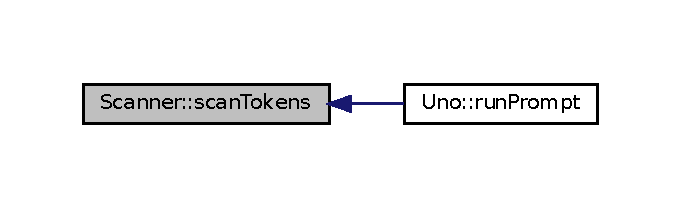
\includegraphics[width=327pt]{classScanner_a38e0f484bb3539944d6809c552f1da0b_icgraph}
\end{center}
\end{figure}


The documentation for this class was generated from the following files\+:\begin{DoxyCompactItemize}
\item 
src/\hyperlink{Scanner_8h}{Scanner.\+h}\item 
src/\hyperlink{Scanner_8cpp}{Scanner.\+cpp}\end{DoxyCompactItemize}

\hypertarget{classToken}{}\section{Token Class Reference}
\label{classToken}\index{Token@{Token}}


{\ttfamily \#include $<$Token.\+h$>$}

\subsection*{Public Member Functions}
\begin{DoxyCompactItemize}
\item 
\hyperlink{classToken_a05effe0dad273695350ae4dd90eec4fc}{Token} (int t, std\+::string lex, int lin)
\item 
std\+::string \hyperlink{classToken_ac5f72b7408cc16946d166963cf1f288d}{to\+String} (void)
\item 
int \hyperlink{classToken_a7ca73dbe9c27e2663f846293aeaff59c}{get\+Type} (void)
\end{DoxyCompactItemize}


\subsection{Detailed Description}


Definition at line 24 of file Token.\+h.



\subsection{Constructor \& Destructor Documentation}
\mbox{\Hypertarget{classToken_a05effe0dad273695350ae4dd90eec4fc}\label{classToken_a05effe0dad273695350ae4dd90eec4fc}} 
\index{Token@{Token}!Token@{Token}}
\index{Token@{Token}!Token@{Token}}
\subsubsection{\texorpdfstring{Token()}{Token()}}
{\footnotesize\ttfamily Token\+::\+Token (\begin{DoxyParamCaption}\item[{int}]{t,  }\item[{std\+::string}]{lex,  }\item[{int}]{lin }\end{DoxyParamCaption})}



Definition at line 4 of file Token.\+cpp.



\subsection{Member Function Documentation}
\mbox{\Hypertarget{classToken_a7ca73dbe9c27e2663f846293aeaff59c}\label{classToken_a7ca73dbe9c27e2663f846293aeaff59c}} 
\index{Token@{Token}!get\+Type@{get\+Type}}
\index{get\+Type@{get\+Type}!Token@{Token}}
\subsubsection{\texorpdfstring{get\+Type()}{getType()}}
{\footnotesize\ttfamily int Token\+::get\+Type (\begin{DoxyParamCaption}\item[{void}]{ }\end{DoxyParamCaption})}



Definition at line 10 of file Token.\+cpp.

Here is the caller graph for this function\+:
\nopagebreak
\begin{figure}[H]
\begin{center}
\leavevmode
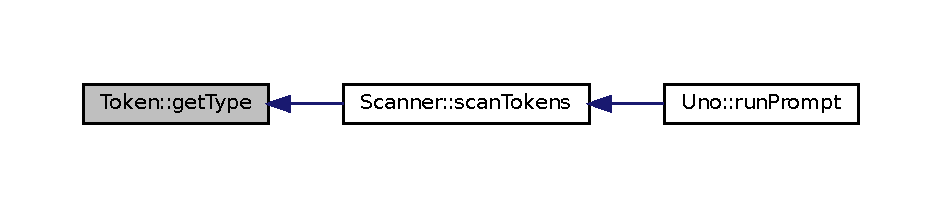
\includegraphics[width=350pt]{classToken_a7ca73dbe9c27e2663f846293aeaff59c_icgraph}
\end{center}
\end{figure}
\mbox{\Hypertarget{classToken_ac5f72b7408cc16946d166963cf1f288d}\label{classToken_ac5f72b7408cc16946d166963cf1f288d}} 
\index{Token@{Token}!to\+String@{to\+String}}
\index{to\+String@{to\+String}!Token@{Token}}
\subsubsection{\texorpdfstring{to\+String()}{toString()}}
{\footnotesize\ttfamily std\+::string Token\+::to\+String (\begin{DoxyParamCaption}\item[{void}]{ }\end{DoxyParamCaption})}



Definition at line 14 of file Token.\+cpp.



The documentation for this class was generated from the following files\+:\begin{DoxyCompactItemize}
\item 
src/\hyperlink{Token_8h}{Token.\+h}\item 
src/\hyperlink{Token_8cpp}{Token.\+cpp}\end{DoxyCompactItemize}

\hypertarget{classUno}{}\section{Uno Class Reference}
\label{classUno}\index{Uno@{Uno}}


{\ttfamily \#include $<$Uno.\+h$>$}

\subsection*{Public Member Functions}
\begin{DoxyCompactItemize}
\item 
\hyperlink{classUno_a82b3a76110117d20bf7d1dd5b9a29e98}{Uno} (void)
\item 
void \hyperlink{classUno_a5fd4f1a9a1688bee5a329dcc191c02f6}{run\+File} (std\+::string path)
\item 
void \hyperlink{classUno_aa690e5403bb1d8a9d3af81b4fa664e1c}{run\+Prompt} (void)
\end{DoxyCompactItemize}


\subsection{Detailed Description}


Definition at line 3 of file Uno.\+h.



\subsection{Constructor \& Destructor Documentation}
\mbox{\Hypertarget{classUno_a82b3a76110117d20bf7d1dd5b9a29e98}\label{classUno_a82b3a76110117d20bf7d1dd5b9a29e98}} 
\index{Uno@{Uno}!Uno@{Uno}}
\index{Uno@{Uno}!Uno@{Uno}}
\subsubsection{\texorpdfstring{Uno()}{Uno()}}
{\footnotesize\ttfamily Uno\+::\+Uno (\begin{DoxyParamCaption}\item[{void}]{ }\end{DoxyParamCaption})}



Definition at line 10 of file Uno.\+cpp.



\subsection{Member Function Documentation}
\mbox{\Hypertarget{classUno_a5fd4f1a9a1688bee5a329dcc191c02f6}\label{classUno_a5fd4f1a9a1688bee5a329dcc191c02f6}} 
\index{Uno@{Uno}!run\+File@{run\+File}}
\index{run\+File@{run\+File}!Uno@{Uno}}
\subsubsection{\texorpdfstring{run\+File()}{runFile()}}
{\footnotesize\ttfamily void Uno\+::run\+File (\begin{DoxyParamCaption}\item[{std\+::string}]{path }\end{DoxyParamCaption})}



Definition at line 14 of file Uno.\+cpp.

\mbox{\Hypertarget{classUno_aa690e5403bb1d8a9d3af81b4fa664e1c}\label{classUno_aa690e5403bb1d8a9d3af81b4fa664e1c}} 
\index{Uno@{Uno}!run\+Prompt@{run\+Prompt}}
\index{run\+Prompt@{run\+Prompt}!Uno@{Uno}}
\subsubsection{\texorpdfstring{run\+Prompt()}{runPrompt()}}
{\footnotesize\ttfamily void Uno\+::run\+Prompt (\begin{DoxyParamCaption}\item[{void}]{ }\end{DoxyParamCaption})}



Definition at line 20 of file Uno.\+cpp.

Here is the call graph for this function\+:
\nopagebreak
\begin{figure}[H]
\begin{center}
\leavevmode
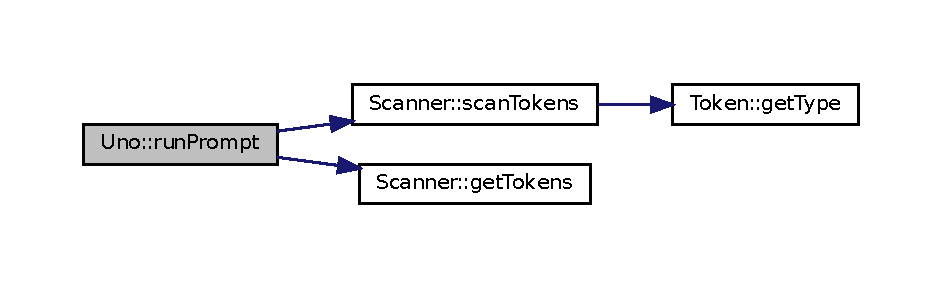
\includegraphics[width=350pt]{classUno_aa690e5403bb1d8a9d3af81b4fa664e1c_cgraph}
\end{center}
\end{figure}


The documentation for this class was generated from the following files\+:\begin{DoxyCompactItemize}
\item 
src/\hyperlink{Uno_8h}{Uno.\+h}\item 
src/\hyperlink{Uno_8cpp}{Uno.\+cpp}\end{DoxyCompactItemize}

\chapter{File Documentation}
\hypertarget{main_8cpp}{}\section{src/main.cpp File Reference}
\label{main_8cpp}\index{src/main.\+cpp@{src/main.\+cpp}}


uno language interpreter.  uno \mbox{[}path\+\_\+to\+\_\+scritp\mbox{]} if a path is given, it\textquotesingle{}s code is run. if uno is called without arguments, an interactive R\+PL is launched.  


{\ttfamily \#include \char`\"{}Uno.\+h\char`\"{}}\newline
{\ttfamily \#include $<$iostream$>$}\newline
Include dependency graph for main.\+cpp\+:
\nopagebreak
\begin{figure}[H]
\begin{center}
\leavevmode
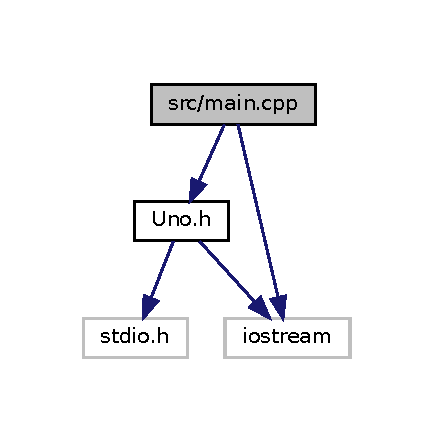
\includegraphics[width=208pt]{main_8cpp__incl}
\end{center}
\end{figure}
\subsection*{Functions}
\begin{DoxyCompactItemize}
\item 
int \hyperlink{main_8cpp_a0ddf1224851353fc92bfbff6f499fa97}{main} (int argc, char $\ast$argv\mbox{[}$\,$\mbox{]})
\end{DoxyCompactItemize}


\subsection{Detailed Description}
uno language interpreter.  uno \mbox{[}path\+\_\+to\+\_\+scritp\mbox{]} if a path is given, it\textquotesingle{}s code is run. if uno is called without arguments, an interactive R\+PL is launched. 



\subsection{Function Documentation}
\mbox{\Hypertarget{main_8cpp_a0ddf1224851353fc92bfbff6f499fa97}\label{main_8cpp_a0ddf1224851353fc92bfbff6f499fa97}} 
\index{main.\+cpp@{main.\+cpp}!main@{main}}
\index{main@{main}!main.\+cpp@{main.\+cpp}}
\subsubsection{\texorpdfstring{main()}{main()}}
{\footnotesize\ttfamily int main (\begin{DoxyParamCaption}\item[{int}]{argc,  }\item[{char $\ast$}]{argv\mbox{[}$\,$\mbox{]} }\end{DoxyParamCaption})}



Definition at line 14 of file main.\+cpp.


\hypertarget{Scanner_8cpp}{}\section{src/\+Scanner.cpp File Reference}
\label{Scanner_8cpp}\index{src/\+Scanner.\+cpp@{src/\+Scanner.\+cpp}}
{\ttfamily \#include \char`\"{}Scanner.\+h\char`\"{}}\newline
{\ttfamily \#include $<$iostream$>$}\newline
{\ttfamily \#include $<$stdlib.\+h$>$}\newline
{\ttfamily \#include $<$string$>$}\newline
{\ttfamily \#include $<$fstream$>$}\newline
{\ttfamily \#include $<$streambuf$>$}\newline
{\ttfamily \#include $<$list$>$}\newline
Include dependency graph for Scanner.\+cpp\+:
\nopagebreak
\begin{figure}[H]
\begin{center}
\leavevmode
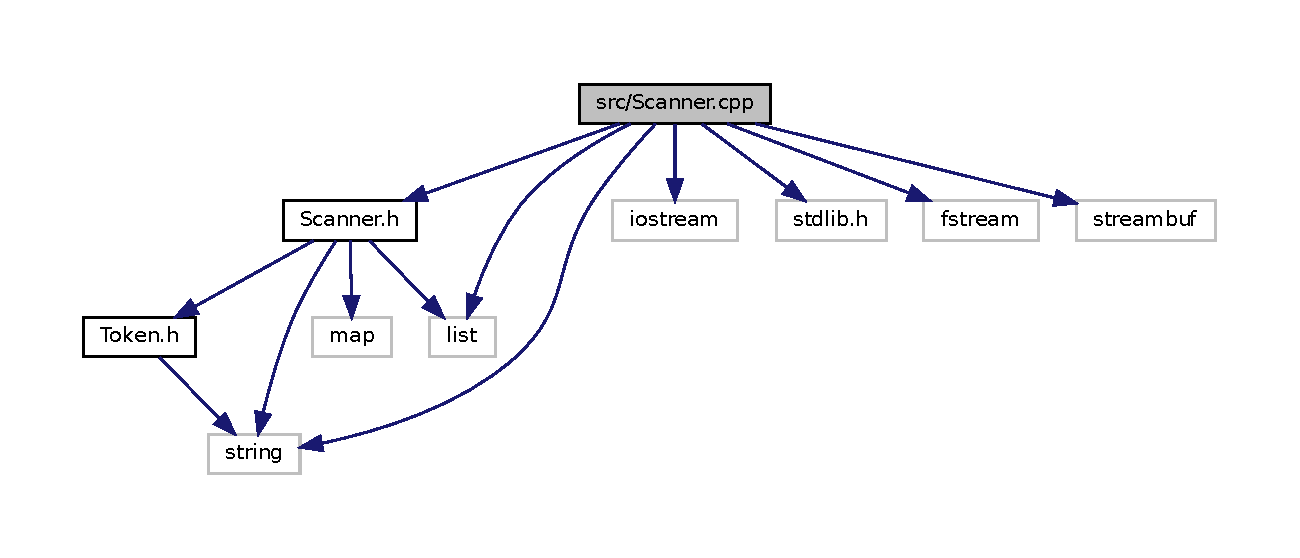
\includegraphics[width=350pt]{Scanner_8cpp__incl}
\end{center}
\end{figure}

\hypertarget{Scanner_8h}{}\section{src/\+Scanner.h File Reference}
\label{Scanner_8h}\index{src/\+Scanner.\+h@{src/\+Scanner.\+h}}
{\ttfamily \#include \char`\"{}Token.\+h\char`\"{}}\newline
{\ttfamily \#include $<$list$>$}\newline
{\ttfamily \#include $<$map$>$}\newline
{\ttfamily \#include $<$string$>$}\newline
Include dependency graph for Scanner.\+h\+:
\nopagebreak
\begin{figure}[H]
\begin{center}
\leavevmode
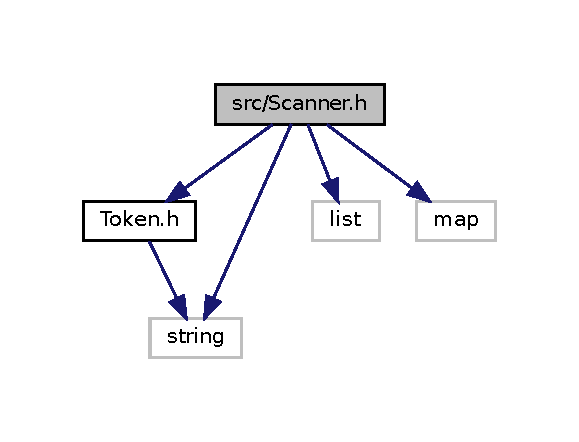
\includegraphics[width=278pt]{Scanner_8h__incl}
\end{center}
\end{figure}
This graph shows which files directly or indirectly include this file\+:
\nopagebreak
\begin{figure}[H]
\begin{center}
\leavevmode
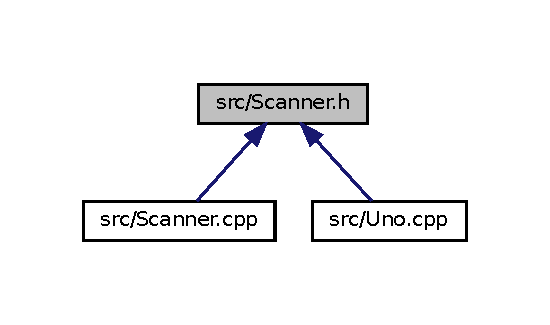
\includegraphics[width=264pt]{Scanner_8h__dep__incl}
\end{center}
\end{figure}
\subsection*{Classes}
\begin{DoxyCompactItemize}
\item 
class \hyperlink{classScanner}{Scanner}
\end{DoxyCompactItemize}

\hypertarget{Token_8cpp}{}\section{src/\+Token.cpp File Reference}
\label{Token_8cpp}\index{src/\+Token.\+cpp@{src/\+Token.\+cpp}}
{\ttfamily \#include \char`\"{}Token.\+h\char`\"{}}\newline
{\ttfamily \#include $<$string$>$}\newline
Include dependency graph for Token.\+cpp\+:
\nopagebreak
\begin{figure}[H]
\begin{center}
\leavevmode
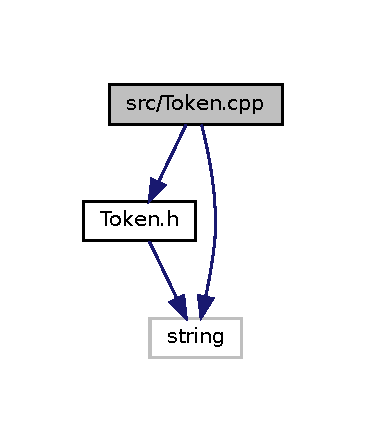
\includegraphics[width=176pt]{Token_8cpp__incl}
\end{center}
\end{figure}

\hypertarget{Token_8h}{}\section{src/\+Token.h File Reference}
\label{Token_8h}\index{src/\+Token.\+h@{src/\+Token.\+h}}
{\ttfamily \#include $<$string$>$}\newline
Include dependency graph for Token.\+h\+:
\nopagebreak
\begin{figure}[H]
\begin{center}
\leavevmode
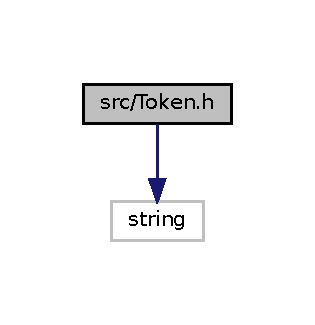
\includegraphics[width=151pt]{Token_8h__incl}
\end{center}
\end{figure}
This graph shows which files directly or indirectly include this file\+:
\nopagebreak
\begin{figure}[H]
\begin{center}
\leavevmode
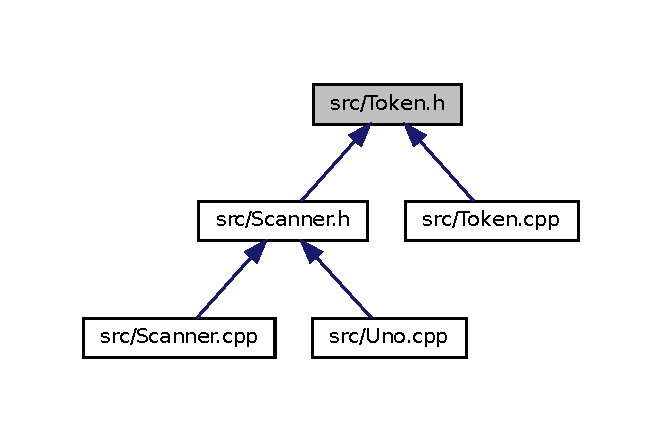
\includegraphics[width=318pt]{Token_8h__dep__incl}
\end{center}
\end{figure}
\subsection*{Classes}
\begin{DoxyCompactItemize}
\item 
class \hyperlink{classToken}{Token}
\end{DoxyCompactItemize}
\subsection*{Typedefs}
\begin{DoxyCompactItemize}
\item 
typedef enum \hyperlink{Token_8h_aa520fbf142ba1e7e659590c07da31921}{Token\+Type} \hyperlink{Token_8h_a223ce5df2488277839246d7ebf52a7f8}{Token\+Type}
\end{DoxyCompactItemize}
\subsection*{Enumerations}
\begin{DoxyCompactItemize}
\item 
enum \hyperlink{Token_8h_aa520fbf142ba1e7e659590c07da31921}{Token\+Type} \{ \newline
\hyperlink{Token_8h_aa520fbf142ba1e7e659590c07da31921aaf335b8436483ffd007e0c1e0ba82374}{L\+E\+F\+T\+\_\+\+P\+A\+R\+EN}, 
\hyperlink{Token_8h_aa520fbf142ba1e7e659590c07da31921aef839b132f4710b720af9322523f64e8}{R\+I\+G\+H\+T\+\_\+\+P\+A\+R\+EN}, 
\hyperlink{Token_8h_aa520fbf142ba1e7e659590c07da31921aad080c3559b964f64a0bf3babee794ae}{L\+E\+F\+T\+\_\+\+B\+R\+A\+CE}, 
\hyperlink{Token_8h_aa520fbf142ba1e7e659590c07da31921a720e33700869f857881e7f50bdfb6943}{R\+I\+G\+H\+T\+\_\+\+B\+R\+A\+CE}, 
\newline
\hyperlink{Token_8h_aa520fbf142ba1e7e659590c07da31921af81277bcd86412fe04bb68718ea09392}{C\+O\+M\+MA}, 
\hyperlink{Token_8h_aa520fbf142ba1e7e659590c07da31921a87fdcd2ffa8f71b49da9e0cfd4fb893f}{D\+OT}, 
\hyperlink{Token_8h_aa520fbf142ba1e7e659590c07da31921af613d73b4e7b570ffd967df4a13c4225}{M\+I\+N\+US}, 
\hyperlink{Token_8h_aa520fbf142ba1e7e659590c07da31921a87fe59ef12c3d13dc2a4d14c9b16c1f9}{P\+L\+US}, 
\newline
\hyperlink{Token_8h_aa520fbf142ba1e7e659590c07da31921a55eebe3c7e08b49cd5969442f4f8c4ce}{S\+E\+M\+I\+C\+O\+L\+ON}, 
\hyperlink{Token_8h_aa520fbf142ba1e7e659590c07da31921aaabdfe7000ca535236502bb0c87ad944}{S\+L\+A\+SH}, 
\hyperlink{Token_8h_aa520fbf142ba1e7e659590c07da31921a9d398750ed310ae69cd070016810e4dc}{S\+T\+AR}, 
\hyperlink{Token_8h_aa520fbf142ba1e7e659590c07da31921a220fa389cdbdc1e8cd33f70c1f793d3c}{B\+A\+NG}, 
\newline
\hyperlink{Token_8h_aa520fbf142ba1e7e659590c07da31921a783d53dd60297984dc8336d5f80cb275}{B\+A\+N\+G\+\_\+\+E\+Q\+U\+AL}, 
\hyperlink{Token_8h_aa520fbf142ba1e7e659590c07da31921a59a84258a4cb9025b567ee5139455029}{E\+Q\+U\+AL}, 
\hyperlink{Token_8h_aa520fbf142ba1e7e659590c07da31921a56bd89f44f205c00adcfe8cb62332f78}{E\+Q\+U\+A\+L\+\_\+\+E\+Q\+U\+AL}, 
\hyperlink{Token_8h_aa520fbf142ba1e7e659590c07da31921a25b5ca2f56d99ba6ffcb5316adac34c1}{G\+R\+E\+A\+T\+ER}, 
\newline
\hyperlink{Token_8h_aa520fbf142ba1e7e659590c07da31921a4495f63771aa2060042a31363e16d4f9}{G\+R\+E\+A\+T\+E\+R\+\_\+\+E\+Q\+U\+AL}, 
\hyperlink{Token_8h_aa520fbf142ba1e7e659590c07da31921a95c736070f99b99eb80d1eac1f4ca60f}{L\+E\+SS}, 
\hyperlink{Token_8h_aa520fbf142ba1e7e659590c07da31921ac7fcbbb467ef6d40ec686d894e26accd}{L\+E\+S\+S\+\_\+\+E\+Q\+U\+AL}, 
\hyperlink{Token_8h_aa520fbf142ba1e7e659590c07da31921a84f8ae2490f9e4bd2321fd21f4b0e807}{I\+D\+E\+N\+T\+I\+F\+I\+ER}, 
\newline
\hyperlink{Token_8h_aa520fbf142ba1e7e659590c07da31921aee847e634a4297b274316de8a8ca9921}{S\+T\+R\+I\+NG}, 
\hyperlink{Token_8h_aa520fbf142ba1e7e659590c07da31921a12a90dfe20486bbe3e075afcd19ef2d0}{N\+U\+M\+B\+ER}, 
\hyperlink{Token_8h_aa520fbf142ba1e7e659590c07da31921a865555c9f2e0458a7078486aa1b3254f}{A\+ND}, 
\hyperlink{Token_8h_aa520fbf142ba1e7e659590c07da31921a8dabc58c34c5df57f2151d6f233d6c15}{C\+L\+A\+SS}, 
\newline
\hyperlink{Token_8h_aa520fbf142ba1e7e659590c07da31921a90d649d830ea440c8b8a56c7ef23c426}{E\+L\+SE}, 
\hyperlink{Token_8h_aa520fbf142ba1e7e659590c07da31921aa1e095cc966dbecf6a0d8aad75348d1a}{F\+A\+L\+SE}, 
\hyperlink{Token_8h_aa520fbf142ba1e7e659590c07da31921a18d8247493ec56714e6beefdf24a546e}{F\+UN}, 
\hyperlink{Token_8h_aa520fbf142ba1e7e659590c07da31921aa809654855caa62449850d9122fd77a8}{F\+OR}, 
\newline
\hyperlink{Token_8h_aa520fbf142ba1e7e659590c07da31921a252802eda493fb6b4a279c4452acb547}{IF}, 
\hyperlink{Token_8h_aa520fbf142ba1e7e659590c07da31921a682466b7669a81b39a8d657274fd4b95}{N\+IL}, 
\hyperlink{Token_8h_aa520fbf142ba1e7e659590c07da31921a96727447c0ad447987df1c6415aef074}{OR}, 
\hyperlink{Token_8h_aa520fbf142ba1e7e659590c07da31921ab107229d44d042caa8ab8df4c8acaa1f}{P\+R\+I\+NT}, 
\newline
\hyperlink{Token_8h_aa520fbf142ba1e7e659590c07da31921a520e09ffec033636dba711f3441cc600}{R\+E\+T\+U\+RN}, 
\hyperlink{Token_8h_aa520fbf142ba1e7e659590c07da31921af877c1dc1b78a33c3c949ed8ac6aac8f}{S\+U\+P\+ER}, 
\hyperlink{Token_8h_aa520fbf142ba1e7e659590c07da31921aac234b49144e47526107d3001284d928}{T\+H\+IS}, 
\hyperlink{Token_8h_aa520fbf142ba1e7e659590c07da31921aa82764c3079aea4e60c80e45befbb839}{T\+R\+UE}, 
\newline
\hyperlink{Token_8h_aa520fbf142ba1e7e659590c07da31921af68346ce0bfce7ab2ca0a240f5132863}{V\+AR}, 
\hyperlink{Token_8h_aa520fbf142ba1e7e659590c07da31921a3278fd035226215822c903790a1eee73}{W\+H\+I\+LE}, 
\hyperlink{Token_8h_aa520fbf142ba1e7e659590c07da31921aae696377c19e507b64e16be78ce3bbdb}{C\+O\+M\+M\+E\+NT}, 
\hyperlink{Token_8h_aa520fbf142ba1e7e659590c07da31921a283fc479650da98250635b9c3c0e7e50}{W\+H\+I\+TE}, 
\newline
\hyperlink{Token_8h_aa520fbf142ba1e7e659590c07da31921adccff14a975cb16ee06d4b5c66e4525c}{E\+O\+FF}, 
\hyperlink{Token_8h_aa520fbf142ba1e7e659590c07da31921a2fd6f336d08340583bd620a7f5694c90}{E\+R\+R\+OR}
 \}
\end{DoxyCompactItemize}


\subsection{Typedef Documentation}
\mbox{\Hypertarget{Token_8h_a223ce5df2488277839246d7ebf52a7f8}\label{Token_8h_a223ce5df2488277839246d7ebf52a7f8}} 
\index{Token.\+h@{Token.\+h}!Token\+Type@{Token\+Type}}
\index{Token\+Type@{Token\+Type}!Token.\+h@{Token.\+h}}
\subsubsection{\texorpdfstring{Token\+Type}{TokenType}}
{\footnotesize\ttfamily typedef enum \hyperlink{Token_8h_aa520fbf142ba1e7e659590c07da31921}{Token\+Type} \hyperlink{Token_8h_aa520fbf142ba1e7e659590c07da31921}{Token\+Type}}



\subsection{Enumeration Type Documentation}
\mbox{\Hypertarget{Token_8h_aa520fbf142ba1e7e659590c07da31921}\label{Token_8h_aa520fbf142ba1e7e659590c07da31921}} 
\index{Token.\+h@{Token.\+h}!Token\+Type@{Token\+Type}}
\index{Token\+Type@{Token\+Type}!Token.\+h@{Token.\+h}}
\subsubsection{\texorpdfstring{Token\+Type}{TokenType}}
{\footnotesize\ttfamily enum \hyperlink{Token_8h_aa520fbf142ba1e7e659590c07da31921}{Token\+Type}}

\begin{DoxyEnumFields}{Enumerator}
\raisebox{\heightof{T}}[0pt][0pt]{\index{L\+E\+F\+T\+\_\+\+P\+A\+R\+EN@{L\+E\+F\+T\+\_\+\+P\+A\+R\+EN}!Token.\+h@{Token.\+h}}\index{Token.\+h@{Token.\+h}!L\+E\+F\+T\+\_\+\+P\+A\+R\+EN@{L\+E\+F\+T\+\_\+\+P\+A\+R\+EN}}}\mbox{\Hypertarget{Token_8h_aa520fbf142ba1e7e659590c07da31921aaf335b8436483ffd007e0c1e0ba82374}\label{Token_8h_aa520fbf142ba1e7e659590c07da31921aaf335b8436483ffd007e0c1e0ba82374}} 
L\+E\+F\+T\+\_\+\+P\+A\+R\+EN&\\
\hline

\raisebox{\heightof{T}}[0pt][0pt]{\index{R\+I\+G\+H\+T\+\_\+\+P\+A\+R\+EN@{R\+I\+G\+H\+T\+\_\+\+P\+A\+R\+EN}!Token.\+h@{Token.\+h}}\index{Token.\+h@{Token.\+h}!R\+I\+G\+H\+T\+\_\+\+P\+A\+R\+EN@{R\+I\+G\+H\+T\+\_\+\+P\+A\+R\+EN}}}\mbox{\Hypertarget{Token_8h_aa520fbf142ba1e7e659590c07da31921aef839b132f4710b720af9322523f64e8}\label{Token_8h_aa520fbf142ba1e7e659590c07da31921aef839b132f4710b720af9322523f64e8}} 
R\+I\+G\+H\+T\+\_\+\+P\+A\+R\+EN&\\
\hline

\raisebox{\heightof{T}}[0pt][0pt]{\index{L\+E\+F\+T\+\_\+\+B\+R\+A\+CE@{L\+E\+F\+T\+\_\+\+B\+R\+A\+CE}!Token.\+h@{Token.\+h}}\index{Token.\+h@{Token.\+h}!L\+E\+F\+T\+\_\+\+B\+R\+A\+CE@{L\+E\+F\+T\+\_\+\+B\+R\+A\+CE}}}\mbox{\Hypertarget{Token_8h_aa520fbf142ba1e7e659590c07da31921aad080c3559b964f64a0bf3babee794ae}\label{Token_8h_aa520fbf142ba1e7e659590c07da31921aad080c3559b964f64a0bf3babee794ae}} 
L\+E\+F\+T\+\_\+\+B\+R\+A\+CE&\\
\hline

\raisebox{\heightof{T}}[0pt][0pt]{\index{R\+I\+G\+H\+T\+\_\+\+B\+R\+A\+CE@{R\+I\+G\+H\+T\+\_\+\+B\+R\+A\+CE}!Token.\+h@{Token.\+h}}\index{Token.\+h@{Token.\+h}!R\+I\+G\+H\+T\+\_\+\+B\+R\+A\+CE@{R\+I\+G\+H\+T\+\_\+\+B\+R\+A\+CE}}}\mbox{\Hypertarget{Token_8h_aa520fbf142ba1e7e659590c07da31921a720e33700869f857881e7f50bdfb6943}\label{Token_8h_aa520fbf142ba1e7e659590c07da31921a720e33700869f857881e7f50bdfb6943}} 
R\+I\+G\+H\+T\+\_\+\+B\+R\+A\+CE&\\
\hline

\raisebox{\heightof{T}}[0pt][0pt]{\index{C\+O\+M\+MA@{C\+O\+M\+MA}!Token.\+h@{Token.\+h}}\index{Token.\+h@{Token.\+h}!C\+O\+M\+MA@{C\+O\+M\+MA}}}\mbox{\Hypertarget{Token_8h_aa520fbf142ba1e7e659590c07da31921af81277bcd86412fe04bb68718ea09392}\label{Token_8h_aa520fbf142ba1e7e659590c07da31921af81277bcd86412fe04bb68718ea09392}} 
C\+O\+M\+MA&\\
\hline

\raisebox{\heightof{T}}[0pt][0pt]{\index{D\+OT@{D\+OT}!Token.\+h@{Token.\+h}}\index{Token.\+h@{Token.\+h}!D\+OT@{D\+OT}}}\mbox{\Hypertarget{Token_8h_aa520fbf142ba1e7e659590c07da31921a87fdcd2ffa8f71b49da9e0cfd4fb893f}\label{Token_8h_aa520fbf142ba1e7e659590c07da31921a87fdcd2ffa8f71b49da9e0cfd4fb893f}} 
D\+OT&\\
\hline

\raisebox{\heightof{T}}[0pt][0pt]{\index{M\+I\+N\+US@{M\+I\+N\+US}!Token.\+h@{Token.\+h}}\index{Token.\+h@{Token.\+h}!M\+I\+N\+US@{M\+I\+N\+US}}}\mbox{\Hypertarget{Token_8h_aa520fbf142ba1e7e659590c07da31921af613d73b4e7b570ffd967df4a13c4225}\label{Token_8h_aa520fbf142ba1e7e659590c07da31921af613d73b4e7b570ffd967df4a13c4225}} 
M\+I\+N\+US&\\
\hline

\raisebox{\heightof{T}}[0pt][0pt]{\index{P\+L\+US@{P\+L\+US}!Token.\+h@{Token.\+h}}\index{Token.\+h@{Token.\+h}!P\+L\+US@{P\+L\+US}}}\mbox{\Hypertarget{Token_8h_aa520fbf142ba1e7e659590c07da31921a87fe59ef12c3d13dc2a4d14c9b16c1f9}\label{Token_8h_aa520fbf142ba1e7e659590c07da31921a87fe59ef12c3d13dc2a4d14c9b16c1f9}} 
P\+L\+US&\\
\hline

\raisebox{\heightof{T}}[0pt][0pt]{\index{S\+E\+M\+I\+C\+O\+L\+ON@{S\+E\+M\+I\+C\+O\+L\+ON}!Token.\+h@{Token.\+h}}\index{Token.\+h@{Token.\+h}!S\+E\+M\+I\+C\+O\+L\+ON@{S\+E\+M\+I\+C\+O\+L\+ON}}}\mbox{\Hypertarget{Token_8h_aa520fbf142ba1e7e659590c07da31921a55eebe3c7e08b49cd5969442f4f8c4ce}\label{Token_8h_aa520fbf142ba1e7e659590c07da31921a55eebe3c7e08b49cd5969442f4f8c4ce}} 
S\+E\+M\+I\+C\+O\+L\+ON&\\
\hline

\raisebox{\heightof{T}}[0pt][0pt]{\index{S\+L\+A\+SH@{S\+L\+A\+SH}!Token.\+h@{Token.\+h}}\index{Token.\+h@{Token.\+h}!S\+L\+A\+SH@{S\+L\+A\+SH}}}\mbox{\Hypertarget{Token_8h_aa520fbf142ba1e7e659590c07da31921aaabdfe7000ca535236502bb0c87ad944}\label{Token_8h_aa520fbf142ba1e7e659590c07da31921aaabdfe7000ca535236502bb0c87ad944}} 
S\+L\+A\+SH&\\
\hline

\raisebox{\heightof{T}}[0pt][0pt]{\index{S\+T\+AR@{S\+T\+AR}!Token.\+h@{Token.\+h}}\index{Token.\+h@{Token.\+h}!S\+T\+AR@{S\+T\+AR}}}\mbox{\Hypertarget{Token_8h_aa520fbf142ba1e7e659590c07da31921a9d398750ed310ae69cd070016810e4dc}\label{Token_8h_aa520fbf142ba1e7e659590c07da31921a9d398750ed310ae69cd070016810e4dc}} 
S\+T\+AR&\\
\hline

\raisebox{\heightof{T}}[0pt][0pt]{\index{B\+A\+NG@{B\+A\+NG}!Token.\+h@{Token.\+h}}\index{Token.\+h@{Token.\+h}!B\+A\+NG@{B\+A\+NG}}}\mbox{\Hypertarget{Token_8h_aa520fbf142ba1e7e659590c07da31921a220fa389cdbdc1e8cd33f70c1f793d3c}\label{Token_8h_aa520fbf142ba1e7e659590c07da31921a220fa389cdbdc1e8cd33f70c1f793d3c}} 
B\+A\+NG&\\
\hline

\raisebox{\heightof{T}}[0pt][0pt]{\index{B\+A\+N\+G\+\_\+\+E\+Q\+U\+AL@{B\+A\+N\+G\+\_\+\+E\+Q\+U\+AL}!Token.\+h@{Token.\+h}}\index{Token.\+h@{Token.\+h}!B\+A\+N\+G\+\_\+\+E\+Q\+U\+AL@{B\+A\+N\+G\+\_\+\+E\+Q\+U\+AL}}}\mbox{\Hypertarget{Token_8h_aa520fbf142ba1e7e659590c07da31921a783d53dd60297984dc8336d5f80cb275}\label{Token_8h_aa520fbf142ba1e7e659590c07da31921a783d53dd60297984dc8336d5f80cb275}} 
B\+A\+N\+G\+\_\+\+E\+Q\+U\+AL&\\
\hline

\raisebox{\heightof{T}}[0pt][0pt]{\index{E\+Q\+U\+AL@{E\+Q\+U\+AL}!Token.\+h@{Token.\+h}}\index{Token.\+h@{Token.\+h}!E\+Q\+U\+AL@{E\+Q\+U\+AL}}}\mbox{\Hypertarget{Token_8h_aa520fbf142ba1e7e659590c07da31921a59a84258a4cb9025b567ee5139455029}\label{Token_8h_aa520fbf142ba1e7e659590c07da31921a59a84258a4cb9025b567ee5139455029}} 
E\+Q\+U\+AL&\\
\hline

\raisebox{\heightof{T}}[0pt][0pt]{\index{E\+Q\+U\+A\+L\+\_\+\+E\+Q\+U\+AL@{E\+Q\+U\+A\+L\+\_\+\+E\+Q\+U\+AL}!Token.\+h@{Token.\+h}}\index{Token.\+h@{Token.\+h}!E\+Q\+U\+A\+L\+\_\+\+E\+Q\+U\+AL@{E\+Q\+U\+A\+L\+\_\+\+E\+Q\+U\+AL}}}\mbox{\Hypertarget{Token_8h_aa520fbf142ba1e7e659590c07da31921a56bd89f44f205c00adcfe8cb62332f78}\label{Token_8h_aa520fbf142ba1e7e659590c07da31921a56bd89f44f205c00adcfe8cb62332f78}} 
E\+Q\+U\+A\+L\+\_\+\+E\+Q\+U\+AL&\\
\hline

\raisebox{\heightof{T}}[0pt][0pt]{\index{G\+R\+E\+A\+T\+ER@{G\+R\+E\+A\+T\+ER}!Token.\+h@{Token.\+h}}\index{Token.\+h@{Token.\+h}!G\+R\+E\+A\+T\+ER@{G\+R\+E\+A\+T\+ER}}}\mbox{\Hypertarget{Token_8h_aa520fbf142ba1e7e659590c07da31921a25b5ca2f56d99ba6ffcb5316adac34c1}\label{Token_8h_aa520fbf142ba1e7e659590c07da31921a25b5ca2f56d99ba6ffcb5316adac34c1}} 
G\+R\+E\+A\+T\+ER&\\
\hline

\raisebox{\heightof{T}}[0pt][0pt]{\index{G\+R\+E\+A\+T\+E\+R\+\_\+\+E\+Q\+U\+AL@{G\+R\+E\+A\+T\+E\+R\+\_\+\+E\+Q\+U\+AL}!Token.\+h@{Token.\+h}}\index{Token.\+h@{Token.\+h}!G\+R\+E\+A\+T\+E\+R\+\_\+\+E\+Q\+U\+AL@{G\+R\+E\+A\+T\+E\+R\+\_\+\+E\+Q\+U\+AL}}}\mbox{\Hypertarget{Token_8h_aa520fbf142ba1e7e659590c07da31921a4495f63771aa2060042a31363e16d4f9}\label{Token_8h_aa520fbf142ba1e7e659590c07da31921a4495f63771aa2060042a31363e16d4f9}} 
G\+R\+E\+A\+T\+E\+R\+\_\+\+E\+Q\+U\+AL&\\
\hline

\raisebox{\heightof{T}}[0pt][0pt]{\index{L\+E\+SS@{L\+E\+SS}!Token.\+h@{Token.\+h}}\index{Token.\+h@{Token.\+h}!L\+E\+SS@{L\+E\+SS}}}\mbox{\Hypertarget{Token_8h_aa520fbf142ba1e7e659590c07da31921a95c736070f99b99eb80d1eac1f4ca60f}\label{Token_8h_aa520fbf142ba1e7e659590c07da31921a95c736070f99b99eb80d1eac1f4ca60f}} 
L\+E\+SS&\\
\hline

\raisebox{\heightof{T}}[0pt][0pt]{\index{L\+E\+S\+S\+\_\+\+E\+Q\+U\+AL@{L\+E\+S\+S\+\_\+\+E\+Q\+U\+AL}!Token.\+h@{Token.\+h}}\index{Token.\+h@{Token.\+h}!L\+E\+S\+S\+\_\+\+E\+Q\+U\+AL@{L\+E\+S\+S\+\_\+\+E\+Q\+U\+AL}}}\mbox{\Hypertarget{Token_8h_aa520fbf142ba1e7e659590c07da31921ac7fcbbb467ef6d40ec686d894e26accd}\label{Token_8h_aa520fbf142ba1e7e659590c07da31921ac7fcbbb467ef6d40ec686d894e26accd}} 
L\+E\+S\+S\+\_\+\+E\+Q\+U\+AL&\\
\hline

\raisebox{\heightof{T}}[0pt][0pt]{\index{I\+D\+E\+N\+T\+I\+F\+I\+ER@{I\+D\+E\+N\+T\+I\+F\+I\+ER}!Token.\+h@{Token.\+h}}\index{Token.\+h@{Token.\+h}!I\+D\+E\+N\+T\+I\+F\+I\+ER@{I\+D\+E\+N\+T\+I\+F\+I\+ER}}}\mbox{\Hypertarget{Token_8h_aa520fbf142ba1e7e659590c07da31921a84f8ae2490f9e4bd2321fd21f4b0e807}\label{Token_8h_aa520fbf142ba1e7e659590c07da31921a84f8ae2490f9e4bd2321fd21f4b0e807}} 
I\+D\+E\+N\+T\+I\+F\+I\+ER&\\
\hline

\raisebox{\heightof{T}}[0pt][0pt]{\index{S\+T\+R\+I\+NG@{S\+T\+R\+I\+NG}!Token.\+h@{Token.\+h}}\index{Token.\+h@{Token.\+h}!S\+T\+R\+I\+NG@{S\+T\+R\+I\+NG}}}\mbox{\Hypertarget{Token_8h_aa520fbf142ba1e7e659590c07da31921aee847e634a4297b274316de8a8ca9921}\label{Token_8h_aa520fbf142ba1e7e659590c07da31921aee847e634a4297b274316de8a8ca9921}} 
S\+T\+R\+I\+NG&\\
\hline

\raisebox{\heightof{T}}[0pt][0pt]{\index{N\+U\+M\+B\+ER@{N\+U\+M\+B\+ER}!Token.\+h@{Token.\+h}}\index{Token.\+h@{Token.\+h}!N\+U\+M\+B\+ER@{N\+U\+M\+B\+ER}}}\mbox{\Hypertarget{Token_8h_aa520fbf142ba1e7e659590c07da31921a12a90dfe20486bbe3e075afcd19ef2d0}\label{Token_8h_aa520fbf142ba1e7e659590c07da31921a12a90dfe20486bbe3e075afcd19ef2d0}} 
N\+U\+M\+B\+ER&\\
\hline

\raisebox{\heightof{T}}[0pt][0pt]{\index{A\+ND@{A\+ND}!Token.\+h@{Token.\+h}}\index{Token.\+h@{Token.\+h}!A\+ND@{A\+ND}}}\mbox{\Hypertarget{Token_8h_aa520fbf142ba1e7e659590c07da31921a865555c9f2e0458a7078486aa1b3254f}\label{Token_8h_aa520fbf142ba1e7e659590c07da31921a865555c9f2e0458a7078486aa1b3254f}} 
A\+ND&\\
\hline

\raisebox{\heightof{T}}[0pt][0pt]{\index{C\+L\+A\+SS@{C\+L\+A\+SS}!Token.\+h@{Token.\+h}}\index{Token.\+h@{Token.\+h}!C\+L\+A\+SS@{C\+L\+A\+SS}}}\mbox{\Hypertarget{Token_8h_aa520fbf142ba1e7e659590c07da31921a8dabc58c34c5df57f2151d6f233d6c15}\label{Token_8h_aa520fbf142ba1e7e659590c07da31921a8dabc58c34c5df57f2151d6f233d6c15}} 
C\+L\+A\+SS&\\
\hline

\raisebox{\heightof{T}}[0pt][0pt]{\index{E\+L\+SE@{E\+L\+SE}!Token.\+h@{Token.\+h}}\index{Token.\+h@{Token.\+h}!E\+L\+SE@{E\+L\+SE}}}\mbox{\Hypertarget{Token_8h_aa520fbf142ba1e7e659590c07da31921a90d649d830ea440c8b8a56c7ef23c426}\label{Token_8h_aa520fbf142ba1e7e659590c07da31921a90d649d830ea440c8b8a56c7ef23c426}} 
E\+L\+SE&\\
\hline

\raisebox{\heightof{T}}[0pt][0pt]{\index{F\+A\+L\+SE@{F\+A\+L\+SE}!Token.\+h@{Token.\+h}}\index{Token.\+h@{Token.\+h}!F\+A\+L\+SE@{F\+A\+L\+SE}}}\mbox{\Hypertarget{Token_8h_aa520fbf142ba1e7e659590c07da31921aa1e095cc966dbecf6a0d8aad75348d1a}\label{Token_8h_aa520fbf142ba1e7e659590c07da31921aa1e095cc966dbecf6a0d8aad75348d1a}} 
F\+A\+L\+SE&\\
\hline

\raisebox{\heightof{T}}[0pt][0pt]{\index{F\+UN@{F\+UN}!Token.\+h@{Token.\+h}}\index{Token.\+h@{Token.\+h}!F\+UN@{F\+UN}}}\mbox{\Hypertarget{Token_8h_aa520fbf142ba1e7e659590c07da31921a18d8247493ec56714e6beefdf24a546e}\label{Token_8h_aa520fbf142ba1e7e659590c07da31921a18d8247493ec56714e6beefdf24a546e}} 
F\+UN&\\
\hline

\raisebox{\heightof{T}}[0pt][0pt]{\index{F\+OR@{F\+OR}!Token.\+h@{Token.\+h}}\index{Token.\+h@{Token.\+h}!F\+OR@{F\+OR}}}\mbox{\Hypertarget{Token_8h_aa520fbf142ba1e7e659590c07da31921aa809654855caa62449850d9122fd77a8}\label{Token_8h_aa520fbf142ba1e7e659590c07da31921aa809654855caa62449850d9122fd77a8}} 
F\+OR&\\
\hline

\raisebox{\heightof{T}}[0pt][0pt]{\index{IF@{IF}!Token.\+h@{Token.\+h}}\index{Token.\+h@{Token.\+h}!IF@{IF}}}\mbox{\Hypertarget{Token_8h_aa520fbf142ba1e7e659590c07da31921a252802eda493fb6b4a279c4452acb547}\label{Token_8h_aa520fbf142ba1e7e659590c07da31921a252802eda493fb6b4a279c4452acb547}} 
IF&\\
\hline

\raisebox{\heightof{T}}[0pt][0pt]{\index{N\+IL@{N\+IL}!Token.\+h@{Token.\+h}}\index{Token.\+h@{Token.\+h}!N\+IL@{N\+IL}}}\mbox{\Hypertarget{Token_8h_aa520fbf142ba1e7e659590c07da31921a682466b7669a81b39a8d657274fd4b95}\label{Token_8h_aa520fbf142ba1e7e659590c07da31921a682466b7669a81b39a8d657274fd4b95}} 
N\+IL&\\
\hline

\raisebox{\heightof{T}}[0pt][0pt]{\index{OR@{OR}!Token.\+h@{Token.\+h}}\index{Token.\+h@{Token.\+h}!OR@{OR}}}\mbox{\Hypertarget{Token_8h_aa520fbf142ba1e7e659590c07da31921a96727447c0ad447987df1c6415aef074}\label{Token_8h_aa520fbf142ba1e7e659590c07da31921a96727447c0ad447987df1c6415aef074}} 
OR&\\
\hline

\raisebox{\heightof{T}}[0pt][0pt]{\index{P\+R\+I\+NT@{P\+R\+I\+NT}!Token.\+h@{Token.\+h}}\index{Token.\+h@{Token.\+h}!P\+R\+I\+NT@{P\+R\+I\+NT}}}\mbox{\Hypertarget{Token_8h_aa520fbf142ba1e7e659590c07da31921ab107229d44d042caa8ab8df4c8acaa1f}\label{Token_8h_aa520fbf142ba1e7e659590c07da31921ab107229d44d042caa8ab8df4c8acaa1f}} 
P\+R\+I\+NT&\\
\hline

\raisebox{\heightof{T}}[0pt][0pt]{\index{R\+E\+T\+U\+RN@{R\+E\+T\+U\+RN}!Token.\+h@{Token.\+h}}\index{Token.\+h@{Token.\+h}!R\+E\+T\+U\+RN@{R\+E\+T\+U\+RN}}}\mbox{\Hypertarget{Token_8h_aa520fbf142ba1e7e659590c07da31921a520e09ffec033636dba711f3441cc600}\label{Token_8h_aa520fbf142ba1e7e659590c07da31921a520e09ffec033636dba711f3441cc600}} 
R\+E\+T\+U\+RN&\\
\hline

\raisebox{\heightof{T}}[0pt][0pt]{\index{S\+U\+P\+ER@{S\+U\+P\+ER}!Token.\+h@{Token.\+h}}\index{Token.\+h@{Token.\+h}!S\+U\+P\+ER@{S\+U\+P\+ER}}}\mbox{\Hypertarget{Token_8h_aa520fbf142ba1e7e659590c07da31921af877c1dc1b78a33c3c949ed8ac6aac8f}\label{Token_8h_aa520fbf142ba1e7e659590c07da31921af877c1dc1b78a33c3c949ed8ac6aac8f}} 
S\+U\+P\+ER&\\
\hline

\raisebox{\heightof{T}}[0pt][0pt]{\index{T\+H\+IS@{T\+H\+IS}!Token.\+h@{Token.\+h}}\index{Token.\+h@{Token.\+h}!T\+H\+IS@{T\+H\+IS}}}\mbox{\Hypertarget{Token_8h_aa520fbf142ba1e7e659590c07da31921aac234b49144e47526107d3001284d928}\label{Token_8h_aa520fbf142ba1e7e659590c07da31921aac234b49144e47526107d3001284d928}} 
T\+H\+IS&\\
\hline

\raisebox{\heightof{T}}[0pt][0pt]{\index{T\+R\+UE@{T\+R\+UE}!Token.\+h@{Token.\+h}}\index{Token.\+h@{Token.\+h}!T\+R\+UE@{T\+R\+UE}}}\mbox{\Hypertarget{Token_8h_aa520fbf142ba1e7e659590c07da31921aa82764c3079aea4e60c80e45befbb839}\label{Token_8h_aa520fbf142ba1e7e659590c07da31921aa82764c3079aea4e60c80e45befbb839}} 
T\+R\+UE&\\
\hline

\raisebox{\heightof{T}}[0pt][0pt]{\index{V\+AR@{V\+AR}!Token.\+h@{Token.\+h}}\index{Token.\+h@{Token.\+h}!V\+AR@{V\+AR}}}\mbox{\Hypertarget{Token_8h_aa520fbf142ba1e7e659590c07da31921af68346ce0bfce7ab2ca0a240f5132863}\label{Token_8h_aa520fbf142ba1e7e659590c07da31921af68346ce0bfce7ab2ca0a240f5132863}} 
V\+AR&\\
\hline

\raisebox{\heightof{T}}[0pt][0pt]{\index{W\+H\+I\+LE@{W\+H\+I\+LE}!Token.\+h@{Token.\+h}}\index{Token.\+h@{Token.\+h}!W\+H\+I\+LE@{W\+H\+I\+LE}}}\mbox{\Hypertarget{Token_8h_aa520fbf142ba1e7e659590c07da31921a3278fd035226215822c903790a1eee73}\label{Token_8h_aa520fbf142ba1e7e659590c07da31921a3278fd035226215822c903790a1eee73}} 
W\+H\+I\+LE&\\
\hline

\raisebox{\heightof{T}}[0pt][0pt]{\index{C\+O\+M\+M\+E\+NT@{C\+O\+M\+M\+E\+NT}!Token.\+h@{Token.\+h}}\index{Token.\+h@{Token.\+h}!C\+O\+M\+M\+E\+NT@{C\+O\+M\+M\+E\+NT}}}\mbox{\Hypertarget{Token_8h_aa520fbf142ba1e7e659590c07da31921aae696377c19e507b64e16be78ce3bbdb}\label{Token_8h_aa520fbf142ba1e7e659590c07da31921aae696377c19e507b64e16be78ce3bbdb}} 
C\+O\+M\+M\+E\+NT&\\
\hline

\raisebox{\heightof{T}}[0pt][0pt]{\index{W\+H\+I\+TE@{W\+H\+I\+TE}!Token.\+h@{Token.\+h}}\index{Token.\+h@{Token.\+h}!W\+H\+I\+TE@{W\+H\+I\+TE}}}\mbox{\Hypertarget{Token_8h_aa520fbf142ba1e7e659590c07da31921a283fc479650da98250635b9c3c0e7e50}\label{Token_8h_aa520fbf142ba1e7e659590c07da31921a283fc479650da98250635b9c3c0e7e50}} 
W\+H\+I\+TE&\\
\hline

\raisebox{\heightof{T}}[0pt][0pt]{\index{E\+O\+FF@{E\+O\+FF}!Token.\+h@{Token.\+h}}\index{Token.\+h@{Token.\+h}!E\+O\+FF@{E\+O\+FF}}}\mbox{\Hypertarget{Token_8h_aa520fbf142ba1e7e659590c07da31921adccff14a975cb16ee06d4b5c66e4525c}\label{Token_8h_aa520fbf142ba1e7e659590c07da31921adccff14a975cb16ee06d4b5c66e4525c}} 
E\+O\+FF&\\
\hline

\raisebox{\heightof{T}}[0pt][0pt]{\index{E\+R\+R\+OR@{E\+R\+R\+OR}!Token.\+h@{Token.\+h}}\index{Token.\+h@{Token.\+h}!E\+R\+R\+OR@{E\+R\+R\+OR}}}\mbox{\Hypertarget{Token_8h_aa520fbf142ba1e7e659590c07da31921a2fd6f336d08340583bd620a7f5694c90}\label{Token_8h_aa520fbf142ba1e7e659590c07da31921a2fd6f336d08340583bd620a7f5694c90}} 
E\+R\+R\+OR&\\
\hline

\end{DoxyEnumFields}


Definition at line 3 of file Token.\+h.


\hypertarget{Uno_8cpp}{}\section{src/\+Uno.cpp File Reference}
\label{Uno_8cpp}\index{src/\+Uno.\+cpp@{src/\+Uno.\+cpp}}
{\ttfamily \#include \char`\"{}Uno.\+h\char`\"{}}\newline
{\ttfamily \#include \char`\"{}Scanner.\+h\char`\"{}}\newline
{\ttfamily \#include $<$iostream$>$}\newline
{\ttfamily \#include $<$stdlib.\+h$>$}\newline
{\ttfamily \#include $<$string$>$}\newline
{\ttfamily \#include $<$fstream$>$}\newline
{\ttfamily \#include $<$streambuf$>$}\newline
Include dependency graph for Uno.\+cpp\+:
\nopagebreak
\begin{figure}[H]
\begin{center}
\leavevmode
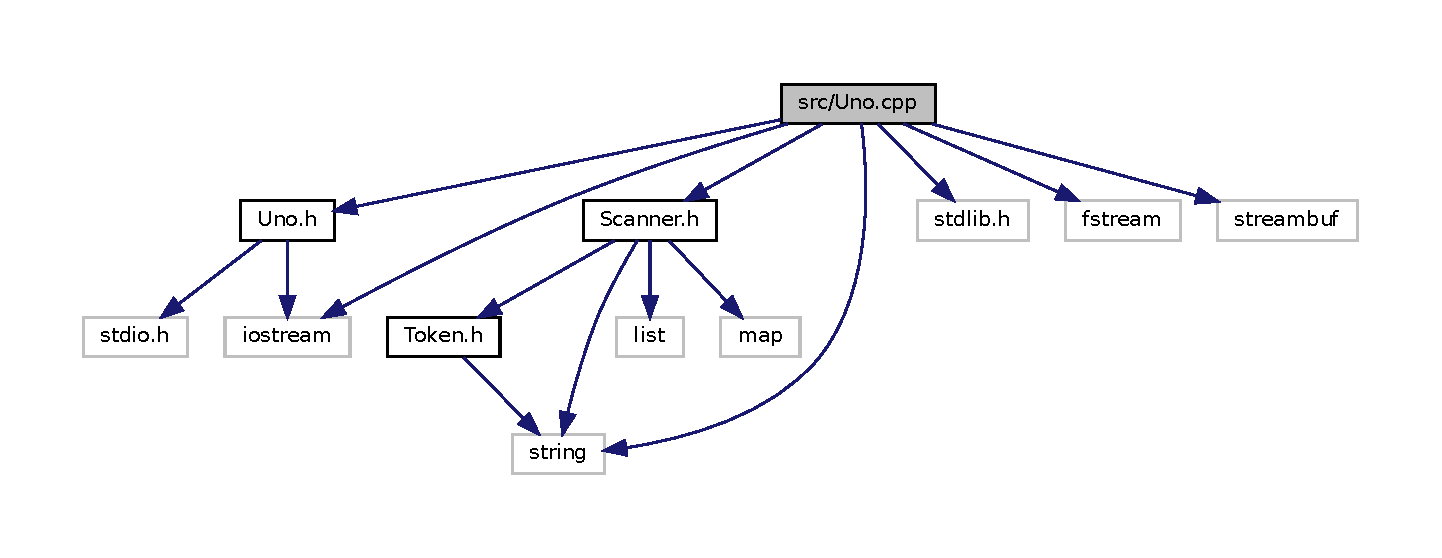
\includegraphics[width=350pt]{Uno_8cpp__incl}
\end{center}
\end{figure}

\hypertarget{Uno_8h}{}\section{src/\+Uno.h File Reference}
\label{Uno_8h}\index{src/\+Uno.\+h@{src/\+Uno.\+h}}
{\ttfamily \#include $<$stdio.\+h$>$}\newline
{\ttfamily \#include $<$iostream$>$}\newline
Include dependency graph for Uno.\+h\+:
\nopagebreak
\begin{figure}[H]
\begin{center}
\leavevmode
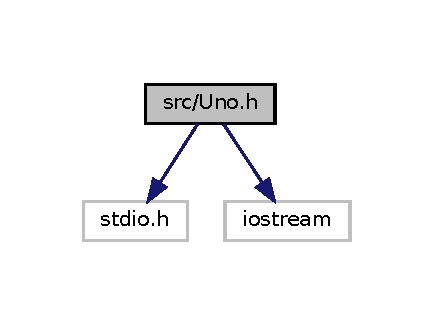
\includegraphics[width=208pt]{Uno_8h__incl}
\end{center}
\end{figure}
This graph shows which files directly or indirectly include this file\+:
\nopagebreak
\begin{figure}[H]
\begin{center}
\leavevmode
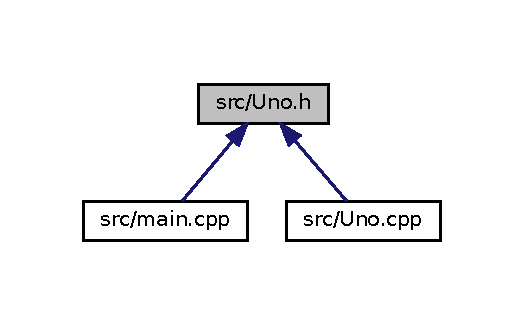
\includegraphics[width=252pt]{Uno_8h__dep__incl}
\end{center}
\end{figure}
\subsection*{Classes}
\begin{DoxyCompactItemize}
\item 
class \hyperlink{classUno}{Uno}
\end{DoxyCompactItemize}

%--- End generated contents ---

% Index
\backmatter
\newpage
\phantomsection
\clearemptydoublepage
\addcontentsline{toc}{chapter}{Index}
\printindex

\end{document}
